% !TEX TS-program = pdflatex
% !TEX encoding = UTF-8 Unicode

% This is a simple template for a LaTeX document using the "article" class.
% See "book", "report", "letter" for other types of document.

\documentclass[11pt]{scrartcl} % use larger type; default would be 10pt

\usepackage[utf8]{inputenc} % set input encoding (not needed with XeLaTeX)

%%% Examples of Article customizations
% These packages are optional, depending whether you want the features they provide.
% See the LaTeX Companion or other references for full information.

%%% PAGE DIMENSIONS
\usepackage{geometry} % to change the page dimensions
\geometry{a4paper} % or letterpaper (US) or a5paper or....
% \geometry{margin=2in} % for example, change the margins to 2 inches all round
% \geometry{landscape} % set up the page for landscape
%   read geometry.pdf for detailed page layout information

\usepackage{graphicx} % support the \includegraphics command and options

% \usepackage[parfill]{parskip} % Activate to begin paragraphs with an empty line rather than an indent

%%% PACKAGES
\usepackage{booktabs} % for much better looking tables
\usepackage{array} % for better arrays (eg matrices) in maths
\usepackage{paralist} % very flexible & customisable lists (eg. enumerate/itemize, etc.)
\usepackage{verbatim} % adds environment for commenting out blocks of text & for better verbatim
\usepackage{subfig} % make it possible to include more than one captioned figure/table in a single float
\usepackage{graphicx}
% These packages are all incorporated in the memoir class to one degree or another...
\usepackage{hyperref}

%%% SECTION TITLE APPEARANCE
\usepackage{sectsty}
\allsectionsfont{\sffamily\mdseries\upshape} % (See the fntguide.pdf for font help)
% (This matches ConTeXt defaults)

%%% ToC (table of contents) APPEARANCE
\usepackage[nottoc,notlof,notlot]{tocbibind} % Put the bibliography in the ToC
\usepackage[titles,subfigure]{tocloft} % Alter the style of the Table of Contents
\renewcommand{\cftsecfont}{\rmfamily\mdseries\upshape}
\renewcommand{\cftsecpagefont}{\rmfamily\mdseries\upshape} % No bold!


\usepackage{amssymb}
\usepackage{amsmath}
\usepackage{mathcomp}
%\usepackage{colortbl}
\usepackage{dsfont}
\usepackage{amsfonts}
\usepackage{cancel}

%%% KV-Diagramme
%\usepackage[ngerman]{babel}
\input kvmacros

%%% Graphen
\usepackage{tikz}
\usetikzlibrary{intersections}
\usetikzlibrary{calc}

% last page
\usepackage{pageslts}

%%% END Article customizations

%%% HEADERS & FOOTERS
\usepackage{fancyhdr} % This should be set AFTER setting up the page geometry
%\usepackage{scrpage2} % Another package (only use fancyhdr or scrpage2)
\pagestyle{fancy} % options: empty , plain , fancy
\renewcommand{\headrulewidth}{1.2pt} % customise the layout...
\renewcommand{\footrulewidth}{0.1pt} % customise the layout...
\lhead{MACHINE LEARNING 1\\Andres Fernandez -- 5692442 -- fr\_andres@msn.com}\chead{}\rhead{Exercise Sheet 6 \\December 12
  , 2016}
\lfoot{}\cfoot{\thepage/\lastpageref{LastPages}}\rfoot{}



%%% THE SYMBOLS FOR ``DEPENDENT'' AND ``INDEPENDENT''
\newcommand{\CI}{\mathrel{\text{\scalebox{1.07}{$\perp\mkern-10mu\perp$}}}} % independent
\newcommand{\nCI}{\cancel{\mathrel{\text{\scalebox{1.07}{$\perp\mkern-10mu\perp$}}}}} % dep
%% THE SYMBOL FOR DOESN'T IMPLY
\newcommand{\notimplies}{%
  \mathrel{{\ooalign{\hidewidth$\not\phantom{=}$\hidewidth\cr$\implies$}}}}

%%% The "real" document content comes below...


\begin{document}

\section*{\\[3mm]Exercise 1}
         {\it ``Completing the square'': suppose you encounter an expression
           \begin{equation}
             \frac{1}{2}w^TCw+b^Tw+a \label{eq1}
           \end{equation}
           with a symmetric square matrix \(C\), vectors \(w\) and \(b\), and constant \(a\). Show that you can bring this into the form
           \begin{equation} \label{eq2}
             \frac{1}{2}(w-m)^TC(w-m)+u
           \end{equation}
           where \(m=-C^{-1}b\) and \(u=a-\frac{1}{2}b^TC^{-1}b\). Hint: insert \(m\) and \(u\) into the expression \ref{eq2} above.}
  

         \subsection*{i)}
         Following the hint, the strategy is to substitute in the expression \ref{eq2} and reformulate it until the equality with \ref{eq1} becomes evident:
         \begin{align*}
           \begin{aligned}
             \frac{1}{2}(w-m)^TC(w-m)+u &= \frac{1}{2}(w+(C^{-1}b))^TC(w+(C^{-1}b))+a-\frac{1}{2}b^TC^{-1}b\\
             ^{(distrib.)}&= \frac{1}{2}(w^T+(C^{-1}b)^T)(Cw+CC^{-1}b))+a-\frac{1}{2}b^TC^{-1}b\\
             ^{(C=C^T,\;\; (AB)^T=B^TA^T,\;\;CC^{-1}=I)}&= \frac{1}{2}(w^T+b^TC^{-1})(Cw+b))+a-\frac{1}{2}b^TC^{-1}b\\
             &= \frac{1}{2}(w^TCw+w^Tb+b^TC^{-1}Cw+b^TC^{-1}b)+a-\frac{1}{2}b^TC^{-1}b\\
             ^{(commut.,\;\;C^{-1}C=I)}&= \frac{1}{2}(w^TCw+w^Tb+b^Tw+b^TC^{-1}b)-\frac{1}{2}b^TC^{-1}b+a\\
             &= \frac{1}{2}(w^TCw+w^Tb+b^Tw)+a\\
             ^{(assoc.)}&= \frac{1}{2}w^TCw+\frac{w^Tb+b^Tw}{2}+a\\
             ^{(w^Tb=b^Tw)}&= \frac{1}{2}w^TCw+b^Tw+a\\
           \end{aligned}
         \end{align*}
         \begin{flushright}
           $\square$\\
         \end{flushright}




\vspace{5mm}
\section*{Exercise 2}
         {\it Now use the method of ’completing the square’ in the exponential to derive the N-dimensional posterior distribution for Bayesian regression. Assume a prior of the form
           \begin{align*}
             p(w) = \mathcal{N}(w|0, \alpha^{-1}I)
           \end{align*}
           And the likelihood
           \begin{align*}
             p(t|X,w,\beta) = \prod_{n=1}^N\mathcal{N}(t_n|w^T\phi(x_n), \beta^{-1})
           \end{align*}
           and show that the posterior is given by
           \begin{align*}
             p(w|t) = \mathcal{N}(w|m_N, S_N)
           \end{align*}
           with
           \begin{align*}
             m_N = \beta S_N \Phi^Tt
           \end{align*}
           and
           \begin{align*}
             S_N^{-1} = \alpha I + \beta \Phi^T\Phi
           \end{align*}
           where \(\Phi\) is the design matrix. }
         
         \subsection*{i)}
         Bayes' theorem states that:
         \begin{align*}
           P(B|A) = \frac{P(A|B)P(B)}{P(A)}
         \end{align*}
         In other words: \(posterior \propto likelihood \times prior\).  So the strategy here is to perform the multiplication between the given likelihood and prior, and perform the necessary transformations until the similarity to the given posterior becomes evident.
         \subsection*{ii)}
         For that, it is convenient to reformulate the likelihood. Remember the formula for the multivariate normal distribution:         
         \begin{align*}
           \begin{aligned}
             \mathcal{N}(\vec{t}\;|\vec{\mu}, \Sigma) = \frac{1}{|2\pi\Sigma|}exp\Big(-\frac{1}{2}(\vec{t}-\vec{\mu})^T\Sigma^{-1} (\vec{t}-\vec{\mu}) \Big)
           \end{aligned}
         \end{align*}
         Now substituting and reformulating the expression for the likelihood (which is unidimensional), yields:
         \begin{align*}
           \begin{aligned}
             p(t|X,w,\beta) &= \prod_{n=1}^N\mathcal{N}(t_n|w^T\phi(x_n), \beta^{-1})\\  
             &= \prod_{n=1}^N\Bigg\{\frac{\beta}{2\pi}exp\bigg(-\frac{1}{2}(t_n-w^T\phi(x_n))\beta (t_n-w^T\phi(x_n)) \bigg) \Bigg\} \\
             &\Big(\frac{\beta}{2\pi}\Big)^Nexp\bigg(-\frac{1}{2}\sum_{n=1}^N\Big\{(t_n-w^T\phi(x_n))\beta (t_n-w^T\phi(x_n))\Big\} \Bigg)
           \end{aligned}
         \end{align*}
         And now the same for the prior:
         \begin{align*}
           \begin{aligned}
             p(w) &= \mathcal{N}(w|0, \alpha^{-1}I) = \frac{1}{|2\pi\alpha^{-1}I|}exp\bigg(-\frac{1}{2}w^T \cdot \alpha I \cdot w \bigg) \\
           \end{aligned}
         \end{align*}

         Now it is possible to multiply both of them by multiplying the normalization terms and adding the exponents:
         \begin{align*}
           \begin{aligned}
             &p(t|X,w,\beta)p(w) =\\
             &\frac{\beta^N}{(2\pi)^N|2\pi\alpha^{-1}I|}exp\bigg(-\frac{1}{2} \bigg( \sum_{n=1}^N\Big\{(t_n-w^T\phi(x_n))\beta (t_n-w^T\phi(x_n))\Big\} + (\vec{w}^{\;\,T} \cdot \alpha I \cdot \vec{w}) \bigg) \Bigg)
           \end{aligned}
         \end{align*}

         \subsection*{iii)}
         As requested, we focus in the exponent, which can be further simplified by introducing the design matrix as defined in the last exercise sheet. By ``completing the square'' it is meant to express the exponent as a function of t, namely a second order polynomial:
         \begin{align*}
           \begin{aligned}
             & -\frac{1}{2} \bigg( \sum_{n=1}^N\Big\{(t_n-w^T\phi(x_n))\beta (t_n-w^T\phi(x_n))\Big\} + (w^T \cdot \alpha I \cdot w)\bigg)\\
             ^{(def. \Phi)}=&-\frac{1}{2} \bigg( (\vec{t}^{\;\,T}-(\vec{w}^{\;\,T}\Phi^T)) \beta(\vec{t}-(\Phi \vec{w}\;\,))  + (w^T \cdot \alpha I \cdot w)\bigg)\\
             ^{(assoc.)}=&-\frac{1}{2} \bigg(\beta (\vec{t}^{\;\,T}t  -  \vec{t}^{\;\,T}\Phi \vec{w}\;\,  - \vec{w}^{\;\,T}\Phi^Tt +  \vec{w}^{\;\,T}\Phi^T\Phi \vec{w}\;\,))  + \alpha(w^T w)\bigg)\\
             ^{( \vec{t}^{\;\,T}\Phi \vec{w}=\vec{w}^{\;\,T}\Phi^Tt)}=&-\frac{1}{2} \bigg(\beta (\vec{t}^{\;\,T}t  -  2\vec{t}^{\;\,T}\Phi \vec{w}\;\, +  \vec{w}^{\;\,T}\Phi^T\Phi \vec{w}\;\,))  + \alpha(w^T w)\bigg)\\
           \end{aligned}
         \end{align*}
         \subsection*{iv)}
         Then, converting the exponent of the posterior as a function of t instead of w yields the same expression:
         \begin{align*}
           \begin{aligned}
             p(w) = \mathcal{N}(w|m_N, S_N) \implies &-\frac{1}{2} (w-m_N)^T S_N^{-1} (w-m_N) \\
             ^{(def.\; m_N)}= &-\frac{1}{2} (w-(\beta S_N \Phi^Tt))^T S_N^{-1} (w-(\beta S_N \Phi^Tt)) \\ %(\alpha I + \beta \Phi^T\Phi)
             ^{(assoc.)}= &-\frac{1}{2} (w^T-(\beta S_N \Phi^Tt)^T) (S_N^{-1}w-(S_N^{-1}\beta S_N \Phi^Tt)) \\
             ^{(A\cdot\beta\cdot A^{-1}=\beta)}= &-\frac{1}{2} (w^T-(\beta S_N \Phi^Tt)^T) (S_N^{-1}w-(\beta \Phi^Tt)) \\
             ^{((ABCD)^T=D^TC^TB^TA^T,\quad \beta^T=\beta)}= &-\frac{1}{2} (w^T-(t^T\Phi S_N^T \beta)) (S_N^{-1}w-(\beta \Phi^Tt)) \\
             ^{(assoc.,\; S_N^T=S_N)}= &-\frac{1}{2} \Big( w^TS_N^{-1}w-w^T\beta \Phi^Tt  - t^T\Phi S_N \beta S_N^{-1}w + t^T\Phi S_N \beta \beta \Phi^Tt \Big) \\
             ^{(w^T\beta\Phi^Tt=t^T\Phi\beta w)}= &-\frac{1}{2} \Big( w^TS_N^{-1}w - 2t^T\Phi\beta w   + t^T\Phi S_N \beta \beta \Phi^Tt \Big) \\
             ^{(def.\; S_N)}= &-\frac{1}{2} \Big( w^T(\alpha I + \beta \Phi^T\Phi)w - 2t^T\Phi\beta w   + t^T\Phi (\alpha I + \beta \Phi^T\Phi)^{-1} \beta \beta \Phi^Tt \Big) \\
             ^{(assoc.)}= &-\frac{1}{2} \Big( w^T(\alpha w + \beta \Phi^T\Phi w) - 2t^T\Phi\beta w   + t^T\Phi (\alpha I + \beta \Phi^T\Phi)^{-1} \beta \beta \Phi^Tt \Big) \\
             ^{(assoc.)}= &-\frac{1}{2} \Big( \alpha w^Tw + w^T\beta \Phi^T\Phi w - 2t^T\Phi\beta w   + t^T\Phi (\alpha I + \beta \Phi^T\Phi)^{-1} \beta \beta \Phi^Tt \Big) \\
             ^{(assoc.)}= &-\frac{1}{2} \Big( \alpha w^Tw + \beta \big(w^T\Phi^T\Phi w - 2t^T\Phi w   + t^T\Phi (\alpha I + \beta \Phi^T\Phi)^{-1} \beta \Phi^Tt \big) \Big) \\
             = &-\frac{1}{2} \Big(t^T\Phi (\alpha I + \beta \Phi^T\Phi)^{-1} \beta \Phi^Tt \big  - 2t^T\Phi w   + \beta \big(w^T\Phi^T\Phi w ) +  \alpha w^Tw\Big) \\
             ^{(commut.)}= &-\frac{1}{2} \Big(t^Tt \big  - 2t^T\Phi w   + \beta \big(w^T\Phi^T\Phi w ) +  \alpha(w^Tw)\Big) \\
           \end{aligned}
         \end{align*}
         \subsection*{v)}
         Now it can be explicitly seen that the expressions at the end of iv) and v) are identical.
         \begin{flushright}
           $\square$\\
         \end{flushright}









         \vspace{5mm}
\section*{Exercise 3}
Please see the  Python2 script {\it fernandez\_blatt6.py} attached to this PDF for the details on how this figures were generated.

           \begin{figure}[ht]
	   \centering
           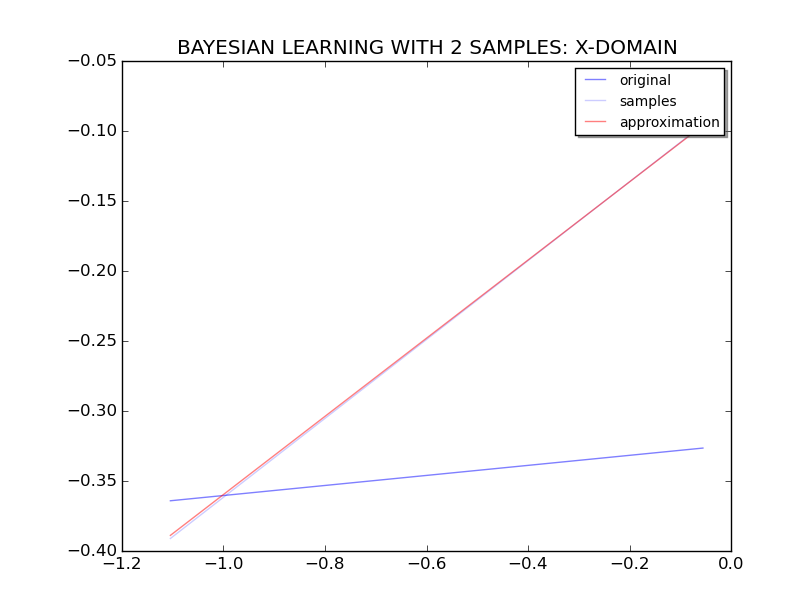
\includegraphics[width=0.7\textwidth, angle=0]{x2.png}
	   \caption{With only two points generated, the posterior isn't able to overcome the noise}
	   \label{fig2}
           \end{figure}
           \begin{figure}[ht]
	   \centering
           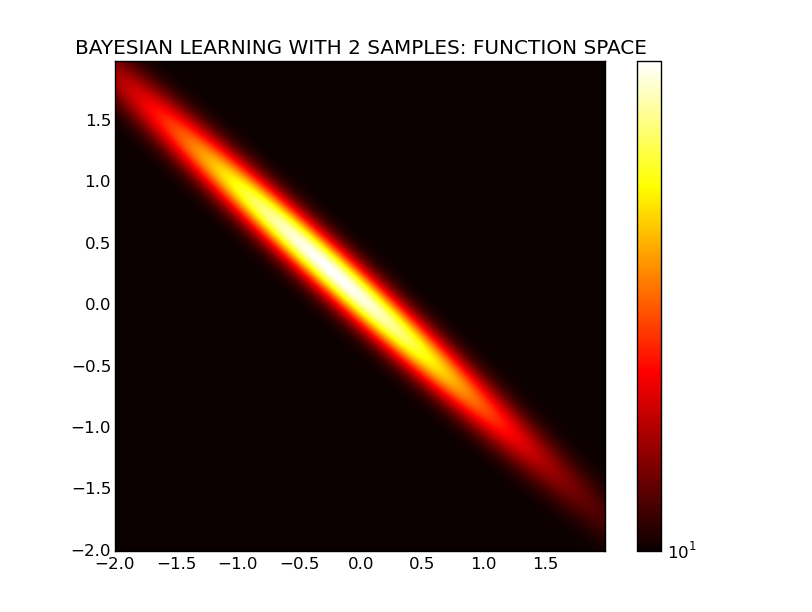
\includegraphics[width=0.7\textwidth, angle=0]{f2.png}
	   \caption{With only two points generated, the prior distribution has predominance. The likelihood provides a linear function space because we have three dimensions, and 2 points, and both of them are multiplied resulting in the observed intersection}
	   \label{fig2}
           \end{figure}
           \begin{figure}[ht]
	   \centering
           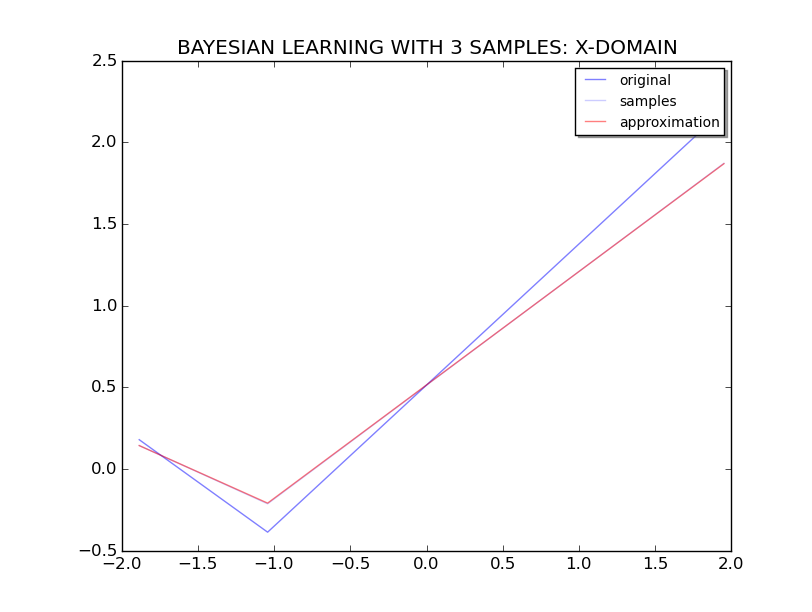
\includegraphics[width=0.7\textwidth, angle=0]{x3.png}
	   \caption{The bayesian estimation progresses greatly in the first steps. This is very useful in small datasets}
	   \label{fig2}
           \end{figure}
           \begin{figure}[ht]
	   \centering
           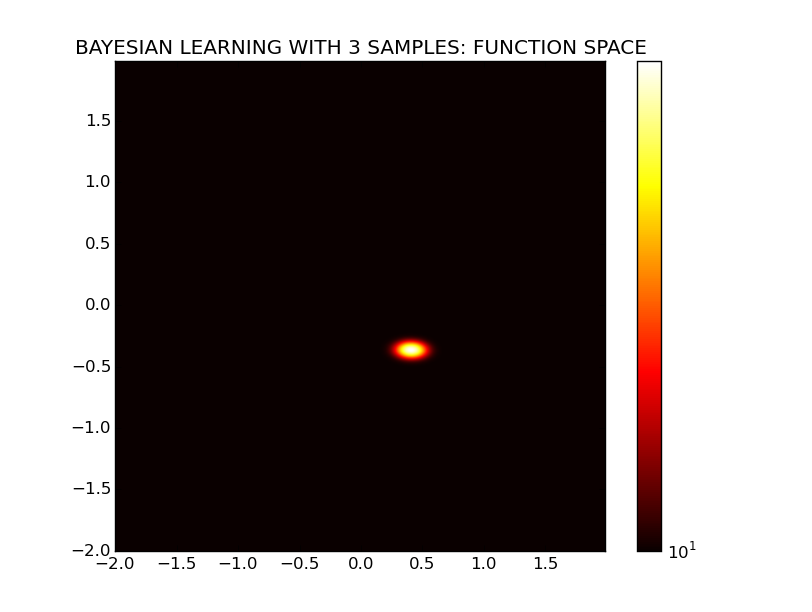
\includegraphics[width=0.7\textwidth, angle=0]{f3.png}
	   \caption{With 3 points it is already possible to limit all dimensions. This plot is the multiplication between the plot before, and the estimation provided by the new point, as it can be seen above in the definition of the likelihood}

	   \label{fig2}
           \end{figure}
           \label{fig2}
           \end{figure}
           \label{fig2}
           \end{figure}
           \begin{figure}[ht]
	   \centering
           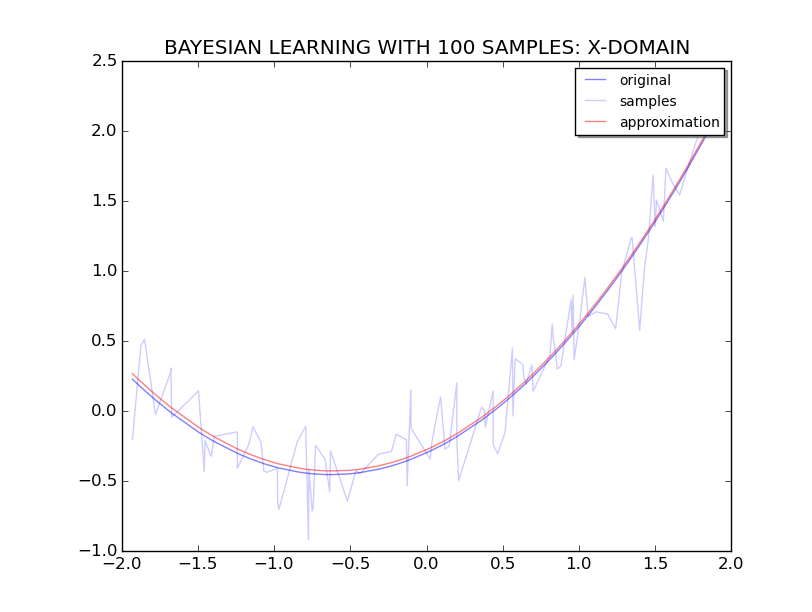
\includegraphics[width=0.7\textwidth, angle=0]{x100.png}
	   \caption{with 100 samples, the approximation is already very percise}
	   \label{fig2}
           \end{figure}
           \begin{figure}[ht]
	   \centering
           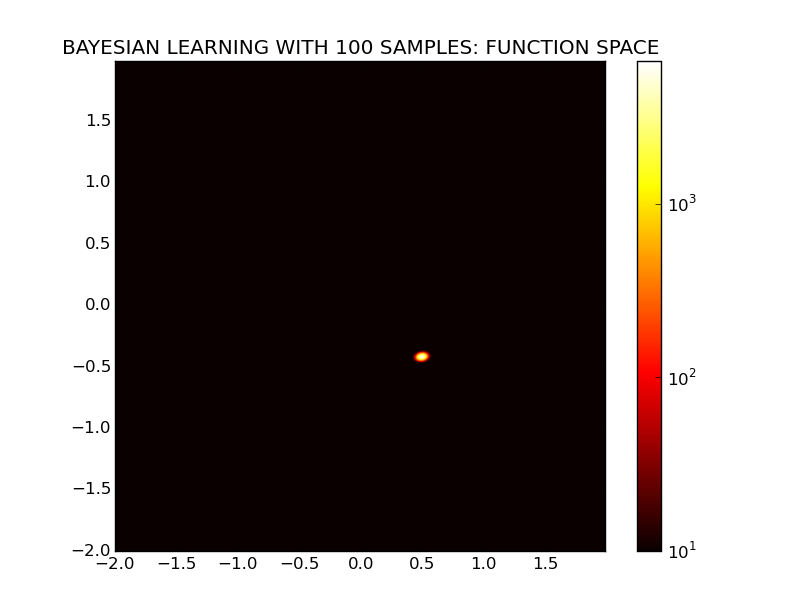
\includegraphics[width=0.7\textwidth, angle=0]{f100.png}
	   \caption{and the feasible function space is extremely reduced, but never to a singular point: the main advantage of bayesian learning is that each possible outcome can be analyzed, and not only the maxima like in the classical ML algorithms. This enable a more explicit formulation of the assumptions and biases, which may help to explain better the existing models}
	   \label{fig2}
           \end{figure}


           

\end{document}




\begin{flushright}
  $\square$\\
\end{flushright}
